\documentclass{article}
\usepackage[utf8]{inputenc}

\usepackage{biblatex}
\addbibresource{refs.bib}

\usepackage{amsmath}
\usepackage{amsfonts}

\usepackage{subcaption}
\usepackage{xcolor}

\usepackage{tikz}
\usetikzlibrary{automata, positioning, arrows}


\tikzset{
    ->,                                         % makes the edges directed
    >=stealth,                                  % makes the arrow heads bold
    %node distance=2cm,                          % specifies the minimum distance between two nodes. Change if necessary.
   % every state/.style={},                 % sets the properties for each ’state’ node
    initial text=$ $,                       % sets the text that appears on the start arrow
}

\title{Linear Algebraic Expression of Weighted Finite State Automata in Speech Recognition}
\author{} % I expect the final document to gather the contribution of many authors including the member of the JSALT FSM and some members of the LISN (e.g. Caio Corro)  
%\date{}


\begin{document}

\maketitle
\abstract{
This an attempt to express of the framework Weighted Finite State Automata in terms of linear algebraic operations.
}
\author{Lucas Ondel}

\tableofcontents

\section{Preliminaries}

\subsection{Semirings}

\paragraph{} A monoid \cite{Golan1999_1} $M = (\mathbb{M}, \odot, e)$ is an algebraic structure over the non-empty set $\mathbb{M}$ with an associative binary function $\odot : \mathbb{M} \times \mathbb{M} \mapsto \mathbb{M}$ whose identity element is $e$, i.e. $(x \odot y) \odot z = x \dot (y \odot z)$ and $e \odot x = x \odot e = x$, $\forall x, y, z \in \mathbb{M}$.  A monoid is commutative is $x \odot y = y \odot x$, $\forall x, y \in \mathbb{M}$

\paragraph{} A semiring \cite{Golan1999_1} $K = (\mathbb{K}, \oplus, \otimes, \bar{0}, \bar{1})$ is an algebraic structure over the non-empty set $\mathbb{K}$ statisfying the following conditions:
\begin{itemize}
    \item $(\mathbb{K}, \oplus, \bar{0})$ is a commutative monoid
    \item $(\mathbb{K}, \otimes, \bar{1})$ is a monoid
    \item $\otimes$ distributes over $\oplus$ from either sides, i.e. $a \otimes (x \oplus y) = (a \otimes x) \oplus (a \otimes y)$ and $(x \oplus y) \otimes a = (x \otimes a) \oplus (y \otimes a)$, $\forall a, x, y \in \mathbb{K}$
    \item $\bar{0} \otimes x = x \otimes \bar{0} = \bar{0}$, $\forall x \in \mathbb{K}$.
\end{itemize}
We say that $K$ is a commutative semiring if $\otimes$ is commutative.

\subsection{Semimodules and $K$-vector space}

Let $K = (\mathbb{K}, \oplus, \otimes, \bar{0}, \bar{1})$ be a semiring. A left $K$-semimodule \cite{Golan1999_2} $S = (\mathbb{S}, K, +, \cdot)$ is a commutative monoid $(
\mathbb{S}, +, \mathbf{0})$ augmented with a function $\cdot : \mathbb{K} \times \mathbb{S} \mapsto \mathbb{S}$, denoted \emph{scalar multiplication} (we write $a \cdot \mathbf{x} = a 
\mathbf{x}$) statisfying the following conditions:
\begin{itemize}
    \item $(a \otimes b) \mathbf{x} = a \otimes (b \mathbf{x})$
    \item $a \otimes (\mathbf{x} + \mathbf{y}) = (a \otimes \mathbf{x}) + (a \otimes \mathbf{y}) $
    \item $(a \oplus b) \mathbf{x} = a \mathbf{x} + b \mathbf{x}$
    \item $\bar{1} \mathbf{x} = \mathbf{x}$
    \item $a \mathbf{0} = \mathbf{0} = \bar{0} \mathbf{x}$,
\end{itemize}
$\forall a, b \in \mathbb{K}$ and $\forall \mathbf{x}, \mathbf{y} \in S$. A right $K$-semimodule follows the same definition with a "right" scalar multiplication.

\paragraph{} Let $K_1$ and $K_2$ be two semirings over the set $\mathbb{K}_1$ and $\mathbb{K}_2$ respectively. We say that $S = (\mathbb{S}, K, +, \cdot)$ is a $(K_1, K_2)$-bisemimodule \cite{Golan1999_2} if $S$ is a left $K_1$-semimodule and a right $K_2$-semimodule and if it satisfies the additional constraint $(a \mathbf{x}) b = a (\mathbf{x} b)$ for all $a \in \mathbb{K}_1$, $\mathbf{x} \in \mathbb{S}$ and $b \in \mathbb{K}_2$.

\paragraph{} We define the $p$-dimensional $K$-vector space as the $(K, K)$-bisemimodule $S = (\mathbb{K}^p, K, +, \cdot)$ constructed as 
\begin{itemize}
    \item $\mathbf{x} + \mathbf{y} = \begin{bmatrix} x_1 \oplus y_1 & \dots & x_d \oplus y_d \end{bmatrix}^\top$, $\forall \mathbf{x}, \mathbf{y} \in \mathbb{K}^p$ 
    \item $a \mathbf{x} = \begin{bmatrix} a \otimes x_1 & \dots & a \otimes x_d \end{bmatrix}^\top$, $\forall a \in \mathbb{K}$ and $\forall \mathbf{x} \in \mathbb{K}^p$.
\end{itemize}
We call an element of $S$ a $K$-\emph{vector}. We define the \emph{dot product}, between two $K$-vectors $\mathbf{x}$ and $\mathbf{y}$, denoted $\mathbf{x}^\top \mathbf{y}$, as 
\begin{align}
    \mathbf{x}^\top \mathbf{y} &= x_1 \otimes y_1 \oplus \dots \oplus x_d \otimes y_d.
\end{align}
Note that the dot product between $K$-vectors is commutative, i.e. $\mathbf{x}^\top \mathbf{y} = \mathbf{y}^\top \mathbf{x}$ only if $K$ is a commutative semiring. 

\paragraph{} The concept of $K$-vector is trivially extended to the one of $K$-matrix (defined over elements of $\mathbb{K}^{p \times q}$). We define the multiplication of a $p \times q$ matrix $\mathbf{A}$ with a $q$-dimensional vector $\mathbf{x}$ as: 
\begin{align}
    \mathbf{A} \mathbf{x} = \mathbf{a}_1 x_1 + \dots + \mathbf{a}_q x_q 
    \label{eq:mv_mul}
\end{align}
where $\mathbf{a}_i$ is the $i$th column of $\mathbf{M}$. Similarly the multiplication of $p$-dimensional transposed $K$-vector $\mathbf{y}^\top$ and a $p \times q$ $K$-matrix $B$ is defined as 
\begin{align}
    \mathbf{y}^\top \mathbf{B} = y_1 \mathbf{b}^1 + \dots + y_p \mathbf{b}^p.
    \label{eq:mvt_mul}
\end{align}
where $\mathbf{b}^i$ is the $i$th row of $\mathbf{B}$. Similarly to the dot product operation, the relation $(\mathbf{A} \mathbf{x})^\top = \mathbf{x}^\top \mathbf{A}^\top$ only holds for all $\mathbf{x} \in \mathbb{K}^q$ if $K$ is a commutative semiring.

\paragraph{} Let $\mathbf{A}$ be a $p \times q$ $K$-matrix, $\mathbf{B}$ a $q \times r$ $K$-matrix. We write the $i$th element of the $j$th column of a ($K$-)matrix $x_j^i$. From \eqref{eq:mv_mul} and $\eqref{eq:mvt_mul}$, we define the $K$-matrix multiplication between $\mathbf{A}$ and $\mathbf{B}$, denoted $\mathbf{A} \mathbf{B}$, the operation producing a $p \times r$ $K$-matrix whose $i$th column is defined as $ \mathbf{a}_1 b_i^1 + \dots + \mathbf{a}_d b_i^d$, or equivalently, whose $j$th row is defined as $a^j_1 \mathbf{b}_1 + \dots + a^j_d \mathbf{b}_d $.

\subsection{Weighted Finite State Automata}

A Weighted Finite State Automaton (WFSA) \cite{Mohri2008} $\mathcal{A} = (\Lambda, Q, I, F, \alpha, \omega, E)$ over a semiring $K$ is a 7-tuple where:
\begin{itemize}
    \item $\Lambda$ is the set of input symbols containing at least the empty sequence $\epsilon$;
    \item $Q$ is the set of states;
    \item $I \subseteq Q$, $F \subseteq Q$ are the sets of initial and final states respectively;
    \item $\alpha : I \mapsto K$, $\omega : F \mapsto K$ are the initial and final weight assignment respectively;
    \item $E \subseteq Q \times \Sigma \times K \times Q$ is a finite set of transitions.
\end{itemize}

\paragraph{} Given transition $e \in E$, $p[e]$ denotes its previous state, $n[e]$ its next state, $w[e]$ its weight and $\lambda[e]$ its label. A path $\boldsymbol{\pi} = e_1 \dots e_k$ is a sequence of transition such that $n[e_{i-1}] = p[e_i]$. We write $|\boldsymbol{\pi}|$ the length of the path, i.e. the number of transitions. The weight of a path $w[\boldsymbol{\pi}] = w[e_1] \otimes \dots \otimes w[e_k]$ is the $\otimes$-product of all its transitions. We say that a string of symbols $\mathbf{x} = x_1 \dots x_k$ is accepted by an automaton $\mathcal{A}$ if there is a path $\boldsymbol{\pi} = e_1 \dots e_l$ in $\mathcal{A}$ with weight $w[\boldsymbol{\pi}] \neq \bar{0}$ such that $\mathbf{x} = \lambda[e_1] \dots \lambda[e_l]$. 

\paragraph{} The weight of an automaton $\mathcal{A}$, denoted $W(\mathcal{A})$, is defined as the $\oplus$-sum of all its accepted path. 

%
\begin{figure}[t] % ’ht’ tells LaTeX to place the figure ’here’ or at the top of the page
    \centering 
    \subcaptionbox{common WFSA.}
        {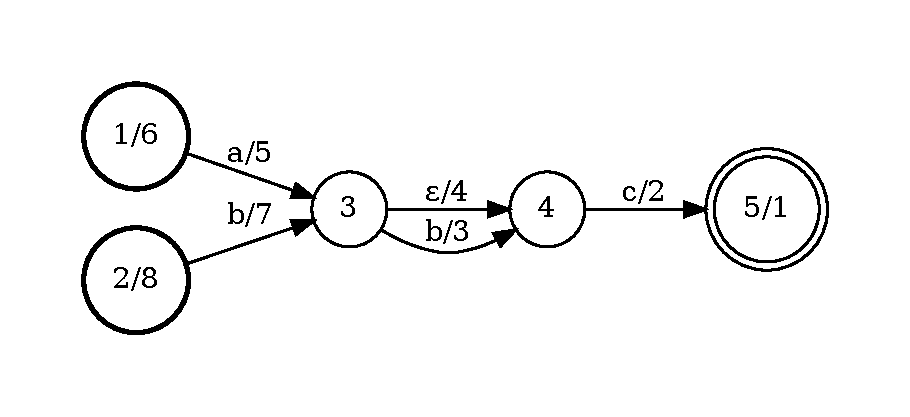
\includegraphics[width=0.7\linewidth]{images/reg_fsa.pdf}}
    \subcaptionbox{\label{simple} simple WFSA.}
        {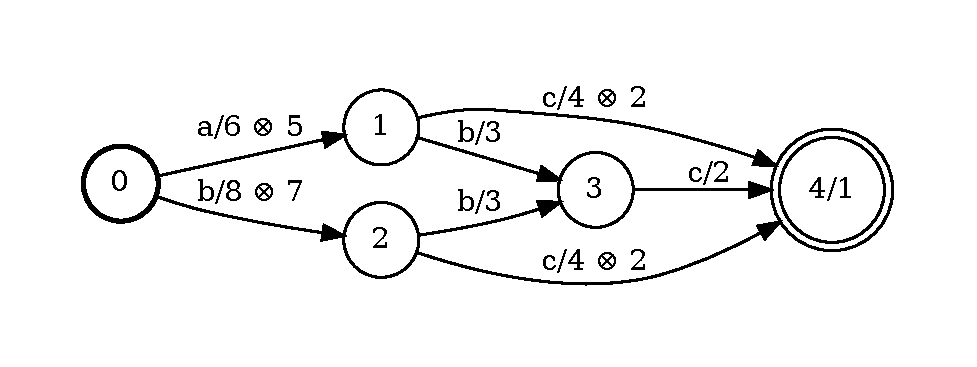
\includegraphics[width=0.7\linewidth]{images/simple_fsa.pdf}}
    \caption{Example of equivalent WFSA accepting the sequences $abc, ac, bbc$, and $bc$.}
    \label{fig:standard_fsa}
\end{figure}
\section{Matrix representation of WFSA}

\subsection{Simple WFSA}

We consider the set of WFSA $\mathbb{A}$ that has a unique initial state (denoted $0$ by convention), has at most one transition between two states, no $\epsilon$ transition and all the arcs going to the same state share the same label, i.e. $\forall e_1, e_2 \in E$, $n[e_1] = n[e_2] \implies \lambda[e_1] = \lambda[e_2]$. By definition, any automaton $\mathcal{A} \in \mathbb{A}$ can be represented as a simple directed graph --- a graph with at most one edge between two vertices. For this reason, we denote such automaton a \emph{simple WFSA}. Remark that simple WFSA are as expressive as standard WFSA since any WFSA can be transformed to an equivalent simple WFSA \textcolor{red}{[PROOF: algorithm / process to convert a general WFSA to a simple WFSA]}. Fig. \ref{fig:wfsa} shows an example of WFSA and an equivalent simple WFSA. 
%
\begin{figure}[t] % ’ht’ tells LaTeX to place the figure ’here’ or at the top of the page
    \centering 
    \subcaptionbox{common WFSA.}
        {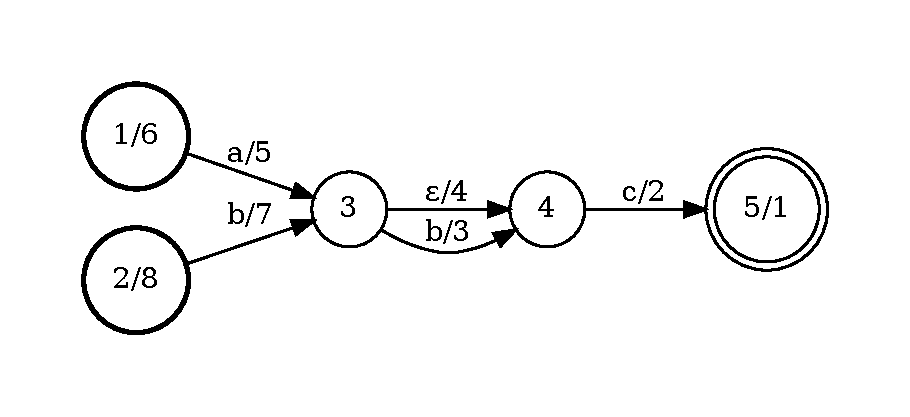
\includegraphics[width=0.7\linewidth]{images/reg_fsa.pdf}}
    \subcaptionbox{\label{simple} simple WFSA.}
        {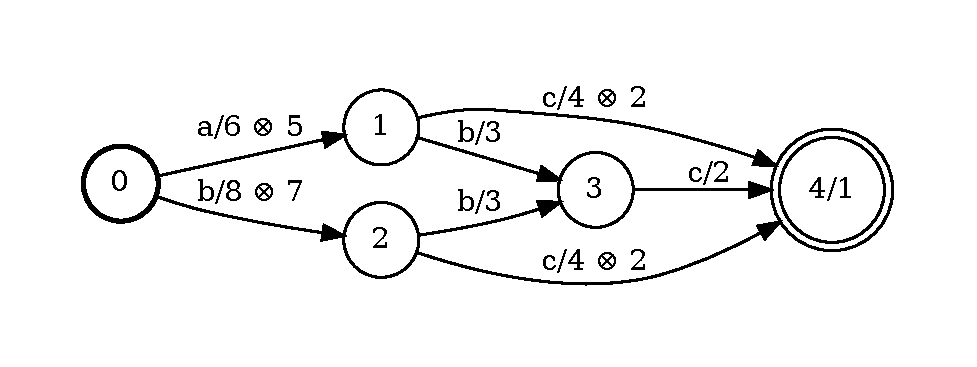
\includegraphics[width=0.7\linewidth]{images/simple_fsa.pdf}}
    \caption{Example of equivalent WFSA accepting the sequences $abc, ac, bbc$, and $bc$.}
    \label{fig:wfsa}
\end{figure}
%

\subsection{Representing simple WFSA in a K-vector space}
\paragraph{} The advantage of simple WFSA is that they can be represented by matrix and vector allowing a linear algebraic treatment of WFSA. Let's consider a simple WFSA $\mathcal{A} = (\Lambda, Q, \{0\}, F, \alpha, \omega, E)$, $\mathcal{A} \in \mathbb{A}$, over the semiring $K = (\mathbb{K}, \oplus, \otimes, \bar{0}, \bar{1})$. We denote $Q' = Q \setminus \{0\}$ the set of states in $\mathcal{A}$ not including the initial state $0$. Let be $S = (\mathbb{K}^{|Q'|}, +, \cdot)$ a $K$-vector space and let be $B$ the standard basis of $S$
\begin{align}
    \mathbf{B} &= \{ \begin{bmatrix} b_{q,1}, \dots, b_{q,|Q'|} \end{bmatrix}^\top : b_{q,i} = \begin{cases} \bar{1} & \text{if $i = q$} \\ \bar{0} & \text{otherwise} \end{cases}\text{, } \forall q \in Q' \}.
\end{align}
The automaton $\mathcal{A}$ can be encoded in terms of an initial weight $K$-vector
\begin{align}
    \boldsymbol{\alpha} &= \sum_{q \in \{e : p[e] = 0, \forall e \in E\}} \alpha(q) \mathbf{b}_{q}, 
\end{align}
a transition $K$-matrix 
\begin{align}
    \mathbf{T} = \sum_{e \in E} w[e] \mathbf{b}_{p[e]} \mathbf{b}_{n[e]}^\top,
\end{align}
a final $K$-vector 
\begin{align}
    \boldsymbol{\omega} &= \sum_{q \in F} \omega(q) \mathbf{b}_{q},
\end{align}
and a vector of label $\boldsymbol{\lambda} \in \Lambda^{|Q'|}$ where $\lambda_q$ is the label associated to the state $q$. The special case of accepting the emtpy string $\epsilon$ is encoded as an extra parameter
\begin{align}
    \rho = \begin{cases}
     \alpha(0) \otimes \omega(0) & \text{if $0 \in F$} \\
     \bar{0} & \text{otherwise}
    \end{cases}.
\end{align}
Hereafter, for a simple WFSA $\mathcal{A}$, we slightly abuse the notation and we write $\mathcal{A} = (\Lambda, Q, \{0\}, F, \alpha, \omega, E)$ or $\mathcal{A} = (\Lambda, Q, \boldsymbol{\alpha}, \mathbf{T}, \boldsymbol{\omega}, \rho, \boldsymbol{\lambda})$ interchangeably.

\subsection{Kernel and Cokernel of $\mathbf{T}$}

We say a state $q \in Q \setminus \{0\} $ is a root state if there is no transition leaving a state in $Q \setminus \{0\}$ and reaching $q$. Stated algebraically, $q$ being a root state implies
\begin{align}
    \forall i \in Q \setminus \{0\}, \;\mathbf{b}_i^\top \mathbf{T} \mathbf{b}_q = \mathbf{0} \implies \mathbf{T} \mathbf{b}_q = \mathbf{0}.
\end{align}
Consequently, the subspace defined the subset of basis associated to the subset of root states of $\mathcal{A}$ is given by the kernel of $\mathbf{T}$, $\text{ker}(\mathbf{T}) = \{ \mathbf{x} : \mathbf{T} \mathbf{x} = \mathbf{0},\; \forall x \in \mathbb{S}\}$. 

\paragraph{} We say a state $q \in Q \setminus \{0\} $ is a leaf state if there is no transition leaving $q$
\begin{align}
    \forall i \in Q \setminus \{0\}, \;\mathbf{b}_q^\top \mathbf{T} \mathbf{b}_i = \mathbf{0} \implies \mathbf{b}_q^\top \mathbf{T} = \mathbf{0}^\top.
\end{align}
Consequently, the subspace defined the subset of basis associated to the subset of leaf states of $\mathcal{A}$ is given by the cokernel of $\mathbf{T}$, $\text{ker}(\mathbf{T}^\top) = \{ \mathbf{x} : \mathbf{x}^\top \mathbf{T} = \mathbf{0}^\top,\; \forall x \in \mathbb{S}\}$. 

\subsection{Evaluating $W(\mathcal{A})$}

Representation of a simple WFSA $\mathcal{A}$ in terms of a K-matrix naturally leads to an easy and efficient way of calculating the sum $W(\mathcal{A})$. Let be $\boldsymbol{\pi}$ an accepted path of length $n$. The weight of a transition $e_i$ from $q_1$ to $q_2$ is given by
\begin{equation}
    w[e_i] = \mathbf{b}_{q_1}^\top \mathbf{T} \mathbf{b}_{q_2}. 
\end{equation}
The $\oplus$-sum of all path of length $2$ leaving $q_1$ and ending in $q_2$ is given by:
\begin{align}
    \Pi_2(\{q_1\}, \{q_2\}) &= \bigoplus_{i \in Q \setminus \{0\}} (\mathbf{b}_{q_1}^\top \mathbf{T} \mathbf{b}_{i}) \otimes (\mathbf{b}_{i}^\top \mathbf{T} \mathbf{b}_{q_2}) \\
    &= \mathbf{b}_{q_1}^\top \mathbf{T} \bigg( \sum_{i \in Q \setminus \{0\}} \mathbf{b}_{i} \mathbf{b}_{i}^\top \bigg) \mathbf{T} \mathbf{b}_{q_2} \\
    &= \mathbf{b}_{q_1}^\top \mathbf{T} \mathbf{T} \mathbf{b}_{q_2}. \label{eq:sum_l2}
\end{align}
Eq. \eqref{eq:sum_l2} can be extended to an arbitrary path length $k$ and arbitrary set of starting states $A \subseteq Q \setminus \{0\}$ and ending states $B \subseteq Q \setminus \{0\}$
\begin{align}
    \Pi_n(A, B) &= \bar{\mathbf{b}}_A^\top  \mathbf{T}^n \bar{\mathbf{b}}_B \label{eq:sum_paths}
\end{align}
where $\bar{\mathbf{b}}_A = \sum_{q \in A} \mathbf{b}_q$, $\bar{\mathbf{b}}_B = \sum_{q \in B} \mathbf{b}_q$ and 
\begin{equation} 
    \mathbf{T}^n = \underbrace{\mathbf{T} \dots \mathbf{T}}_{n \text{ times}}.
\end{equation}
is the $k$th power of the $K$-matrix $\mathbf{T}$. With \eqref{eq:sum_paths} and taking into account the initial and final weights $\boldsymbol{\alpha}$ and $\boldsymbol{\omega}$, one can express $W(\mathcal{A})$ as the $\oplus$-sum of all the path of length 0, 1, 2, ...
\begin{align}
    W(\mathcal{A}) &= \rho \oplus \bigoplus_{n=1}^\infty \boldsymbol{\alpha}^\top \mathbf{T}^n \boldsymbol{\omega}. \label{eq:total_sum}.
\end{align}

\begin{align}
    W(\mathcal{A}) &= \rho \oplus \boldsymbol{\alpha}^\top ( \mathbf{T}^0 + \mathbf{T}^1 + \mathbf{T}^2 + ...   )\boldsymbol{\omega} \label{eq:total_sum}
\end{align}

\begin{align}
    \mathbf{T}_C &= \mathbf{M}^\top (\mathbf{T}_A \otimes \mathbf{T}_B) \mathbf{M}
\end{align}


\paragraph{} Eq. \eqref{eq:total_sum} naturally lends itself to a recursive computation: 
\begin{align}
    \mathbf{u}_1 &= \boldsymbol{\alpha} \\
    \mathbf{u}_n &= (\mathbf{u}_{n-1}^\top \mathbf{T})^\top \label{eq:forward_rec}
\end{align}
leading to 
\begin{align}
    W(\mathcal{A}) &= \rho \oplus \bigoplus_{n=1}^\infty \mathbf{u}_n^\top \boldsymbol{\omega}.
\end{align}

\paragraph{} Eq. \eqref{eq:forward_rec} leads to an interesting observation: a simple WFSA can be interpreted as linear dynamical system in a $K$-vector space representing the states of the automaton. The recursion to evaluate of the automaton's weight $W(\mathcal{A})$ is analog to evaluate a trajectory from the initial configuration $\boldsymbol{\alpha}$. An illustration is given in Fig. \ref{fig:ldyn_wfsa}.
%
\begin{figure}[t] 
    \centering 
    \subcaptionbox{simple WFSA $\mathcal{A}$ with initial weights parameterized by $\sigma$.}
        {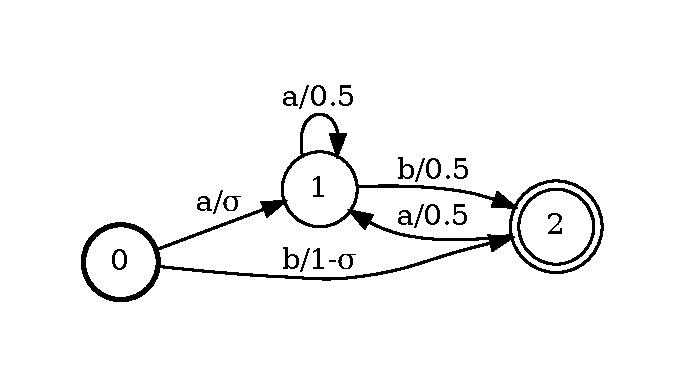
\includegraphics[width=0.49\linewidth]{images/swfsa.pdf}}
    \subcaptionbox{\label{simple} $K$-vector space representing the state-space of $\mathcal{A}$.}
        {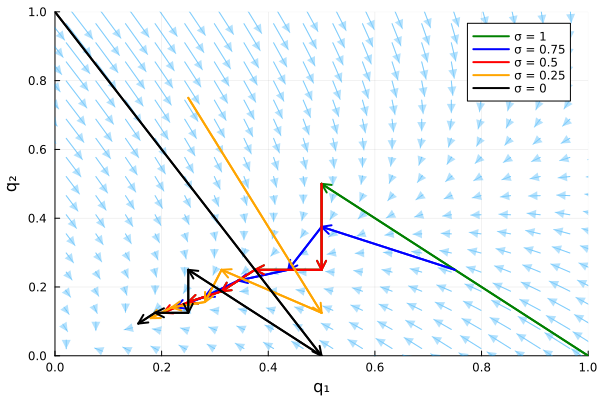
\includegraphics[width=0.49\linewidth]{images/dyn_system.png}}
    \caption{Visualisation of trajectories as a function of $\sigma$ taken while computing $W(\mathcal{A})$. The blue arrows in background represent the linear dynamical system induced by the transition matrix}
    \label{fig:ldyn_wfsa}
\end{figure}

\subsection{Acyclic Simple WFSA}

By definition, an acyclic simple WFSA $\mathcal{A}$ can only accept path whose length are less than $|Q \setminus \{0\}|$. This implies that there exists a $k \leq |Q \setminus \{0\}| + 1$ such that 
\begin{align}
    \forall \boldsymbol{\alpha}, \boldsymbol{\omega} \in \mathbb{S}^{|Q \setminus \{0\}|} \; \boldsymbol{\alpha}^\top \mathbf{T}^k \boldsymbol{\omega} = \bar{0}.
\end{align}
Consequently, the transition matrix of $\mathcal{A}$ is nilpotent, i.e. $\mathbf{T}^k = \mathbf{0}$ for some $k$.

\paragraph{} The consequence of this result is that, as one would expect, the $\oplus$-sum in \eqref{eq:total_sum} is finite for acyclic simple WFSA
\begin{align}
    W(\mathcal{A}) &= \rho \oplus \bigoplus_{n=1}^{\max_{\boldsymbol{\pi}} |\boldsymbol{\pi}|} \boldsymbol{\alpha}^\top \mathbf{T}^n \boldsymbol{\omega}.
\end{align}
It allows therefore to define a another recursion going backward 
\begin{align}
    \mathbf{v}_n &= \boldsymbol{\omega} \\
    \mathbf{v}_n &= \mathbf{T} \mathbf{v}_{n+1} \\
    W_n(\mathcal{A}) &= \rho \oplus \boldsymbol{\alpha}^\top \mathbf{v}_n.
    \label{eq:sum_paths_rec_swfsa_b}
\end{align}
Finally both recursions can be combined, for $1 < m < n$ we have
\begin{equation}
    W_n(\mathcal{A}) = \rho \oplus \mathbf{u}_m^\top 
    \mathbf{v}_{m+1}.
\end{equation}
 
%  We define its simple graph representation $L(\mathcal{A})$   
% constructed in the following way:
% \begin{enumerate}
%     \item for every edge $e \in E$ make a new labeled state in $L(\mathcal{A})$ with label $\lambda[e]$;
%     \item for every edge $e \in E$ we assign an initial weight $\alpha(p[e]) \otimes w[e]$ and a final weight $\omega(n[e])$ to the corresponding vertex in $L(\mathcal{A})$; 
%     \item for every two edges $e_1, e_2 \in E$ such that $n[e_1] = p[e_2]$ make a directed edge in $L(\mathcal{A})$ with weight $w[e_2]$ between their corresponding vertices;
%     \item for every pair of edge $e_1, e_2$ in $L(\mathcal{A})$ connected head-to-tail in a vertex with label $\epsilon$ add a new edge from $p[e_1]$ to $p[e_2]$ with weight $w[e_1] \otimes w[e_2]$;
%     \item for every vertex $v$ in $L(\mathcal{A})$ with label $\epsilon$, remove $v$ from $L(\mathcal{A})$  and for every pair of edge $e_1, e_2$ connected head-to-tail in $v$ add a new edge from with weight $w[e_1] \otimes w[e_2]$. 
% \end{enumerate}
% An illustration of $L(\mathcal{A})$ where $\mathcal{A}$ is defined as in Fig. \ref{fig:standard_fsa} is shown in Fig. \ref{fig:simplegraph_wfsa}.
%

\subsection{Weighted Pushdown Automata}

\begin{align}
    \mathbf{v}_n^{(1)} &= \mathbf{T}^{(1) \top} \mathbf{v}_{n-1}^{(1)} + \mathbf{\bar{P}}^{(2)} \mathbf{u}_{n-1}^{(2)} \\
    \vdots \\
    \mathbf{v}_n^{(i)} &= \big( \mathbf{1}_{N^{(i-1)}} \otimes \mathbf{T}^{(i) \top} \big) \mathbf{v}_{n-1}^{(i)} + \mathbf{P}^{(i-1)} \mathbf{w}_{n-1}^{(i-1)}  + \mathbf{\bar{P}}^{(i+1)} \mathbf{u}_{n-1}^{(i+1)}  \\
    \vdots \\
    \mathbf{v}_n^{(d)} &= \big( \mathbf{1}_{N^{(d-1)}} \otimes \mathbf{T}^{(d) \top} \big) \mathbf{v}_{n-1}^{(d)} + \mathbf{P}^{(d-1)} \mathbf{w}_{n-1}^{(d-1)} 
\end{align}


\begin{align}
    \mathbf{w}_n^{(1)} &= \mathbf{v}^{(1)}_n \\
    \mathbf{w}_n^{(i)} &= \mathbf{P}^{(i-1)} \mathbf{w}_{n}^{(i-1)}  \\
    \mathbf{u}_n^{(d)} &= \mathbf{u}^{(d)}_n \\
    \mathbf{u}_n^{(i)} &= \mathbf{\bar{P}}^{(i+1)} \mathbf{u}_{n}^{(di+1)}
\end{align}

\section{Basic operations on simple WFSA}


\section{WFSA-based loss function}

Let $\mathbf{X} = \begin{bmatrix} \mathbf{x}_1, \dots{x}_N \end{bmatrix}$, $\mathbf{x}_i \in \mathbb{R}^D$, be a input sequence of features and let $\mathbf{Y} = \phi(\mathbf{X}) = \begin{bmatrix} \mathbf{y}_1, \dots, \mathbf{y}_M \end{bmatrix}$, $\mathbf{y}_i \in \mathbb{R}^{D'}$ be the output sequence of an arbitrary mapping $\phi$ (typically a neural network).

We defined:
\begin{align}
    p(\mathbf{X}, \mathbf{y}) &= \frac{\sum_{\mathbf{z}}\exp \{ \phi(\mathbf{X}, \mathbf{z}) + \psi(\mathbf{z}, \mathbf{y}) \} }{Z} \\
    Z &= \int_{\mathbf{X}} \sum_{\mathbf{z}} \sum_\mathbf{y} \exp \{ \phi(\mathbf{X}, \mathbf{z}) + \psi(\mathbf{z}, \mathbf{y}) \} \text{d}\mathbf{X}
\end{align}

\subsection{Mutual Information}

\begin{align}
    I(\mathbf{X}; \mathbf{y}) &= \mathbb{E}_{p(\mathbf{X}, \mathbf{y})} \Big[ \ln \frac{p(\mathbf{X}, \mathbf{y})}{p(\mathbf{X})p(\mathbf{y})} \Big]
\end{align}
where
\begin{align}
     \frac{p(\mathbf{X}, \mathbf{y})}{p(\mathbf{X})} &= \frac{\sum_{\mathbf{z}}\exp \{ \phi(\mathbf{X}, \mathbf{z}) + \psi(\mathbf{z}, \mathbf{y}) \} }{\sum_{\mathbf{y}} \sum_{\mathbf{z}}\exp \{ \phi(\mathbf{X}, \mathbf{z}) + \psi(\mathbf{z}, \mathbf{y}) \}} \frac{Z}{Z} \\
     &= \frac{\sum_{\mathbf{z}}\exp \{ \phi(\mathbf{X}, \mathbf{z}) + \psi(\mathbf{z}, \mathbf{y}) \} }{\sum_{\mathbf{y}} \sum_{\mathbf{z}}\exp \{ \phi(\mathbf{X}, \mathbf{z}) + \nu(\mathbf{z}) \}}
\end{align}
where the function $\nu$ is defined such that
\begin{align}
     \exp \{ \nu(\mathbf{z}) \} &= \sum_{\mathbf{y}} \exp \{ \psi(\mathbf{z}, \mathbf{y}) \}.
\end{align}
Therefore the MI objective function becomes:
\begin{align}
    I(\mathbf{X}; \mathbf{y}) &= \mathbb{E}_{p(\mathbf{X}, \mathbf{y})} \Big[\ln \Big( \sum_{\mathbf{z}}\exp \{ \phi(\mathbf{X}, \mathbf{z}) + \psi(\mathbf{z}, \mathbf{y}) \Big) - \ln \Big( \sum_{\mathbf{y}} \sum_{\mathbf{z}}\exp \{ \phi(\mathbf{X}, \mathbf{z}) + \nu(\mathbf{z}) \Big)  \Big] + \text{const}
\end{align}
\subsection{Backpropagation through WFSA}

We turn now to the problem of estimating the gradient of $W(\mathcal{A})$ --- where $\mathcal{A}$ is an acyclic simple WFSA $\mathcal{A}$ over a semiring $K$ --- with respect to the parameters $\boldsymbol{\theta} = \{ \boldsymbol{\alpha}, \boldsymbol{\omega},  \mathbf{T}, \boldsymbol{\omega}, \rho\}$. The gradient depends on the semiring $K$ and therefore we cannot obtain a unique solution. Instead we restrict ourselves to semirings that are isomorphic to the  probability semiring. 

\paragraph{} Let $P = (\mathbb{R}^+, +, \cdot, 0, 1)$ be the probability semiring and let $K = (\mathbb{K}, \oplus, \otimes, \bar{0}, \bar{1})$ be a semiring isomorphic to $P$ with the morphism $f : K \mapsto P$. Let $\mathcal{A}_K = (\Lambda, Q, I, F, \alpha, \omega, E_K)$ be a simple WFSA over the semiring $K$ and 
\begin{align}
    \mathcal{A}_P &= (\Lambda, Q, I, F, f \circ \alpha, f \circ \omega, E_P) \\
    E_P &= \{ (s, l, d, f(w)) : \forall (s, l, d, w) \in E_K\}
\end{align} 
where, in this context, $\circ$ is the function composition operator. Informally, $\mathcal{A}_P$ is the automaton $\mathcal{A}_K$ with weights converted to the probability semiring. 

\paragraph{} Using the isomorphic nature of $\mathcal{A}_K$ and $\mathcal{A}_P$, we can derive a practical formula of the gradient:
\begin{align}
    \frac{\partial W(\mathcal{A}_K)}{\partial \boldsymbol{\theta}_K} &= \frac{\partial f^{-1}( W(\mathcal{A}_P) ) }{\partial \boldsymbol{\theta}_K} \\
    &= \frac{\partial f^{-1}}{\partial W(\mathcal{A}_P)} \frac{\partial W(\mathcal{A}_P)}{\partial \boldsymbol{\theta}_P}, \label{eq:grad_sum_paths}
\end{align}
where $\boldsymbol{\theta}_K = \{ \boldsymbol{\alpha}_K,  \mathbf{T}_K, \boldsymbol{\omega}_K, \rho_K \}$ and $\boldsymbol{\theta}_P = \{ \boldsymbol{\alpha}_P,  \mathbf{T}_P, \boldsymbol{\omega}_P, \rho_P \}$ are the parameters of 
$\mathcal{A}_K$ and $\mathcal{A}_P$ respectively. Since $W(\mathcal{A}_P)$ is defined in the real semiring its gradient can evaluated easily:
\begin{align}
    W(\mathcal{A}_P) &= \rho + \sum_{n=1}^{k-1} \boldsymbol{\alpha}_P^{\top} \mathbf{T}_P^{n} \boldsymbol{\omega}_p. \label{eq:grad_sum_paths_real}
\end{align}
From \eqref{eq:grad_sum_paths_real} we get
\begin{align}
    \frac{\partial W(\mathcal{A}_P)}{\partial \boldsymbol{\alpha}} &= \sum_{n=1}^{k-1} \mathbf{T}_P^n \boldsymbol{\omega}_P \\
    \frac{\partial W(\mathcal{A}_P)}{\partial \mathbf{T}_P} &= \sum_{r=0}^{k - 2} \sum_{q=0}^{k-2-r} \mathbf{T}_P^{r \top} \boldsymbol{\alpha}_P \boldsymbol{\omega}_P^\top \mathbf{T}_P^{q \top} \label{eq:grad_adj_matrix}\\
    \frac{\partial W(\mathcal{A}_P)}{\partial \boldsymbol{\omega}} &= \sum_{n=1}^{k-1} (\boldsymbol{\alpha}^\top \mathbf{T}_P^n)^\top \\
    \frac{\partial W(\mathcal{A}_P)}{\partial \rho} &= 1,
\end{align}
where we have used the identity
\begin{align}
    \frac{\partial \mathbf{a}^\top \mathbf{X}^d \mathbf{b}}{\partial \mathbf{X}} &= \sum_{r=0}^{d-1} \mathbf{X}^{r\top} \mathbf{a} \mathbf{b}^\top \mathbf{X}^{d - 1 - r \top}
\end{align}
in \eqref{eq:grad_adj_matrix}.



\section{Specific Topologies }

Let $\mathbf{X} \in \mathbb{R}^{D \times N}$ be a sequence of $N$ $D$-dimensional vectors, let $\Lambda$ be a set of symbols and let $\mathbf{H} = g(\mathbf{X})$,  $\mathbf{H} \in \mathbb{R}^{L \times M}$, be the output a weighting function $g$ (e.g. a neural network) which takes $\mathbf{X}$ as input sequence and outputs a sequence of $M$ $|\Lambda|$-dimensional vectors such that $\mathbf{h}_{m} = g_m ( \mathbf{X})$. The weights $\mathbf{H}$ may be interpreted as the weights of a SWFSA whose structure may be defined in various ways. In the rest of this section we explore some commonly used structure for speech recognition. 

\subsection{Time-synchronous WFSA}

Let $\mathbf{H}$ have length  $M = N + 1$ that is for every time step $\mathbf{x}_n$ there is a corresponding weighting vector $\mathbf{h}_n$ and a final weighting $\mathbf{h}_{N+1}$. We define a time-synchronous WFSA over a semiring $K$ as $\mathcal{A} = (\Lambda, \{0, \dots, N \times |\Lambda| \}, \boldsymbol{\alpha}, \mathbf{T}, \boldsymbol{\omega}, \bar{0}, \boldsymbol{\lambda})$ where:

\begin{align}
    \boldsymbol{\alpha} &= \begin{bmatrix} \mathbf{h}_1 \\ \mathbf{0} \end{bmatrix} & \boldsymbol{\omega} &= \begin{bmatrix} \mathbf{0} \\ \mathbf{h}_{N+1} \end{bmatrix} \\
    \mathbf{T} &= \begin{bmatrix}
        \mathbf{0} & \mathbf{1} \mathbf{h}_2^\top & \mathbf{0} & \dots\\
        \mathbf{0} & \mathbf{0} & \mathbf{1} \mathbf{h}_3^\top & \ddots \\
        \vdots & & \ddots & \ddots 
    \end{bmatrix} & \boldsymbol{\lambda} &= \mathbf{1}_{N} \otimes \begin{bmatrix} 
        l_1 \\ \vdots \\ l_{|\Lambda|}
    \end{bmatrix}, \; \forall l \in \Lambda.
\end{align}

\subsubsection{Intersection}
The intersection of a time synchronous WFSA $A$ with an arbitrary WFSA $B$ yields another time-synchronous WFSA $C = A \cap B = (\Lambda, Q_C, \boldsymbol{\alpha}_C, \mathbf{T}_C
, \boldsymbol{\omega}_C, \bar{0}, \boldsymbol{\lambda}_C)$ defined as such:
\begin{align}
    Q &= \{0, 1, \dots, N|\Lambda| \} \\
    \boldsymbol{\alpha}_C &= \begin{bmatrix}
        (\mathbf{M}^\top \mathbf{h}_1) \circ \boldsymbol{\alpha}_B \\ \mathbf{0}
    \end{bmatrix} \qquad \boldsymbol{\omega}_C = \begin{bmatrix}
        \mathbf{0} \\(\mathbf{M}^\top \mathbf{h}_{N+1}) \circ \boldsymbol{\omega}_B 
    \end{bmatrix} \\
    \mathbf{T} &= \begin{bmatrix}
        \mathbf{0} & \mathbf{1} (\mathbf{M}^\top \mathbf{h}_2)^\top \circ \mathbf{T}_B & \mathbf{0} & \dots\\
        \mathbf{0} & \mathbf{0} & \mathbf{1} (\mathbf{M}^\top \mathbf{h}_3)^\top \circ \mathbf{T}_B & \ddots \\
        \vdots & \vdots & \vdots & \ddots 
    \end{bmatrix} \quad \boldsymbol{\lambda} = \begin{bmatrix} 
        \boldsymbol{\lambda}_B \\ \boldsymbol{\lambda}_B \\ \dots
    \end{bmatrix}.
\end{align}
In practice it is usually not necessary to evaluate the elements of $C$ as one can evaluate $W(C)$ directly as follows:
\begin{align}
    \mathbf{u}_1 &= (\mathbf{M}^\top \mathbf{h}_1) \circ \boldsymbol{\alpha}_B \\
    \mathbf{u}_n &= (\mathbf{M}^\top \mathbf{h}_n) \circ (\mathbf{T}_B^\top \mathbf{u}_{n-1}) \\
    W(C) &= \mathbf{u}_N^\top [(\mathbf{M}^\top \mathbf{h}_{N+1}) \circ \boldsymbol{\omega}_B]
\end{align}

\begin{figure}[t] 
    \centering 
    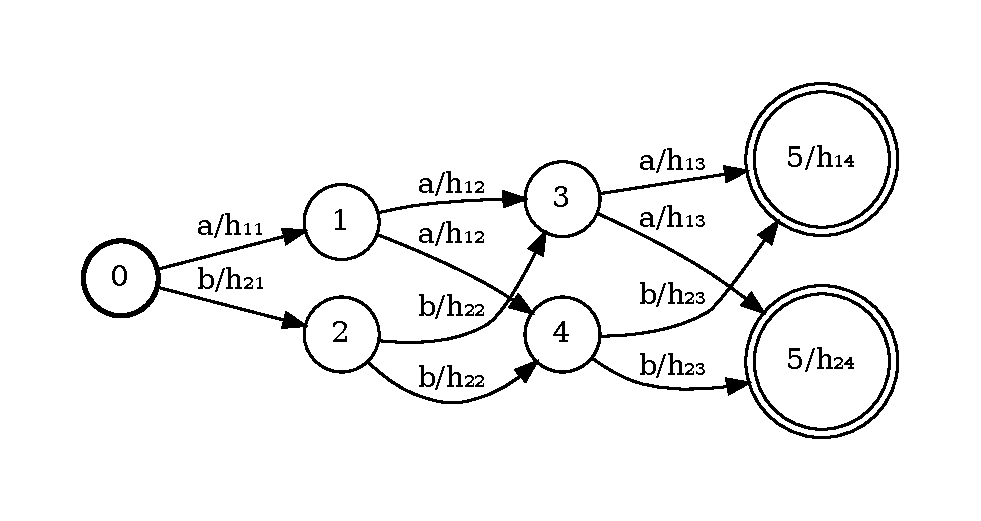
\includegraphics[width=0.7\linewidth]{images/dense.pdf}
    \label{fig:dense_fsa}
\end{figure}

\begin{align}
    \mathbf{v}_{N+1} &= (\mathbf{M}^\top \mathbf{h}_{N+1}) \circ \boldsymbol{\omega}_B \\
    \mathbf{v}_{n} &= \mathbf{T}_B [ (\mathbf{M}^\top \mathbf{h}_n) \circ \mathbf{v}_{n+1}] \\
    W(C) &= [(\mathbf{M}^\top \mathbf{h}_1) \circ \boldsymbol{\alpha}_B]^\top \mathbf{v}_2
\end{align}
Generally, for any $n$, $1 < n < N+1$, 
\begin{align}
    W(C) &= \mathbf{u}_n^\top \mathbf{v}_{n+1}
\end{align}

\paragraph{Gradient}

\begin{align} 
    % \mathbf{g}_{n} &= \mathbf{M}^\top \mathbf{h}_{n} \\
    \mathbf{g}_{n} &= \exp \{ \mathbf{x}_n \} = \mathbf{M}^\top \mathbf{h}_n\\
    \frac{\partial \ln W(C)}{\partial \mathbf{x}_{n}} &= \frac{1}{W(C)} \frac{\partial W(C)}{\partial \mathbf{g}_n} \frac{\partial \mathbf{g}_n}{\partial \mathbf{x}_n} \\ %\frac{\partial \mathbf{h}_n}{\partial \mathbf{x}_n} 
    &= \frac{1}{W(C)} (\mathbf{u}_n \circ \mathbf{v}_{n+1})
\end{align}

\begin{align} 
    \mathbf{h}_n &= \exp \{ \mathbf{x}_n \} \\
    \mathbf{g}_{n} &= \mathbf{M}^\top \mathbf{h}_{n} \\
    \frac{\partial \ln W(C)}{\partial \mathbf{x}_{n}} &= \frac{1}{W(C)} \frac{\partial W(C)}{\partial \mathbf{g}_n} \frac{\partial \mathbf{g}_n}{\partial \mathbf{h}_n} \frac{\partial \mathbf{h}_n}{\partial \mathbf{x}_n} \\
    &= \frac{1}{W(C)} \exp \{ \mathbf{x}_n \} \circ \mathbf{M} \Big( (\mathbf{T}_B^\top \mathbf{u}_{n-1}) \circ \mathbf{v}_{n+1} \Big)
\end{align}

\subsubsection{Current Implementation of $\nabla_\mathbf{H} W(C)$}
\paragraph{Forward Recursion}
\begin{align}
    \mathbf{u}_1 &= \boldsymbol{\alpha}_B \\
    \mathbf{u}_n &= \mathbf{T}_B^\top [ (\mathbf{M}^\top \mathbf{h}_{n-1}) \circ \mathbf{u}_{n-1} ] \\
    W(C) &= [(\mathbf{M}^\top \mathbf{h}_N) \circ \mathbf{u}_N]^\top [(\mathbf{M}^\top \mathbf{h}_{N+1}) \circ \boldsymbol{\omega}_B]
\end{align}

\paragraph{Backward Recursion}
\begin{align}
    \mathbf{v}_{N} &= (\mathbf{M}^\top \mathbf{h}_{N+1}) \circ  \boldsymbol{\omega}_B \\
    \mathbf{v}_n &= \mathbf{T}_B [ (\mathbf{M}^\top \mathbf{h}_{n+1}) \circ \mathbf{v}_{n+1} ] \\
    W(C) &= [(\mathbf{M}^\top \mathbf{h}_1) \circ \boldsymbol{\alpha}_B]^\top \mathbf{v}_1 \\
    W(C) &= [(\mathbf{M}^\top \mathbf{h}_n) \circ \mathbf{u}_n]^\top \mathbf{v}_n
\end{align}

\paragraph{Gradient}
\begin{align}
    \mathbf{h}_n &= \exp\{\mathbf{x}_n\} \\
    \frac{\partial W(C)}{\partial \mathbf{h}_n} &= 
        \frac{\partial}{\partial \mathbf{h}_n}
        [(\mathbf{M}^\top \mathbf{h}_n) \circ \mathbf{u}_n]^\top \mathbf{v}_n \\
    &= \mathbf{M}(\mathbf{u}_n \circ \mathbf{v}_n)\\
    \frac{\partial W(C)}{\partial \mathbf{h}_{N+1}} &= 
        \frac{\partial}{\partial \mathbf{h}_{N+1}}
        [(\mathbf{M}^\top \mathbf{h}_n) \circ \mathbf{u}_n]^\top
        [(\mathbf{M}^\top \mathbf{h}_{N+1}) \circ  \boldsymbol{\omega}_B] \\
    &= \mathbf{M}[(\mathbf{M}^\top\mathbf{h}_N) \circ \mathbf{u}_N \circ \boldsymbol{\omega}_B]\\
    \frac{\partial \log\left(W(C)\right)}{\partial \mathbf{x}_n} &= 
        \frac{\partial \log\left(W(C)\right)}{\partial W(C)}
        \left[
            \frac{\partial \mathbf{h}_n}{\mathbf{x}_n}
        \right]^\top 
        \frac{\partial W(C)}{\partial \mathbf{h}_n}\\
    &= \frac{1}{W(C)} \exp\{\mathbf{x}_n\} \circ \mathbf{M}(\mathbf{u}_n \circ \mathbf{v}_n)
\end{align}

\printbibliography

\end{document}
